\documentclass[../m2r-report.tex]{subfile}

\subsection{Finite Graphs}
\label{sec:1.1}

Whilst Ramsey's original paper \cite{Ramsey1930} is concerned with a problem of logic, Erd{\"o}s and 
Szekeres \cite{Erdos1935} reformulated his work in a graph theoretical sense. The idea of proving 
the existence of regular substructure within an apparently chaotic superstructure
is immediately applicable to graphs. The content of this section primarily follows 
that of Bollobás's book \textit{Modern Graph Theory} \cite{Bollobas1998}.

In the graph below, we partition the edges into two disjoint sets: red lines and blue 
lines. In turns out that no matter how we partition our edges, we will always get
red triangles or blue triangles. In this particular partition, we get two 
red triangles.

\begin{figure}[h]
\begin{center}
    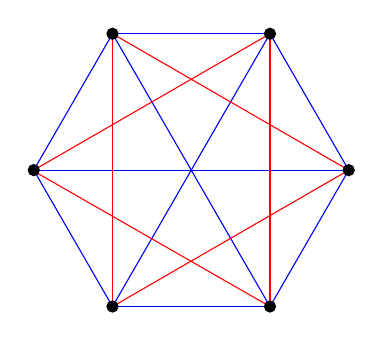
\begin{tikzpicture}
        \draw [blue] (0,0) -- (2,0);
        \draw [blue] (2,0) -- (3,1.7321);
        \draw [blue] (3,1.7321) -- (2,3.4641);
        \draw [blue] (2,3.4641) -- (0,3.4641);
        \draw [blue] (0,3.4641) -- (-1,1.7321);
        \draw [blue] (-1,1.7321) -- (0,0);
        \draw [blue] (0,0) -- (2,3.4641);
        \draw [blue] (3,1.7321) -- (-1,1.7321);
        \draw [blue] (2,0) -- (0,3.4641);

        \draw [red] (0,0) -- (3,1.7321);
        \draw [red] (3,1.7321) -- (0,3.4641);
        \draw [red] (0,3.4641) -- (0,0);
        \draw [red] (2,0) -- (2,3.4641);
        \draw [red] (2,3.4641) -- (-1,1.7321);
        \draw [red] (-1,1.72,0) -- (2,0);

        \filldraw (0,0) circle (2pt);
        \filldraw (2,0) circle (2pt);
        \filldraw (3,1.7321) circle (2pt);
        \filldraw (2,3.4641) circle (2pt);
        \filldraw (0,3.4641) circle (2pt);
        \filldraw (-1,1.7321) circle (2pt);
    \end{tikzpicture}

\end{center}

\caption{2 red triangles within a graph of 6 vertices}
\end{figure}

Before continuing, we first need to state some notation and definitions\cite{Graham1990}.

For $n,k\in \Z^+$, and any non-empty set $X$, let

\begin{align*}%\label{eq:bracketDef}
[n] &= \{1, 2,\ldots, n\},\\
X^{(k)} &= \{Y:Y\subseteq X, |Y|=k\}.
\end{align*}

\begin{definition}[Graph]

    A \textit{graph G} is an ordered pair of disjoint countable sets $(V,E)$ such that $E$ 
    is a subset of $V^{(2)}$, the set of unordered pairs of $V$. We call $V$ the 
    set of vertices, and $E$ the set of edges. The \textit{order}
    of $G$ is the number of vertices, i.e $|V|$.

\end{definition}

\begin{definition}[Complete graph]

    We say a graph $G:=(V,E)$ is \textit{complete} if $E=V^{(2)}$. Intuitively, a graph 
    is complete if every pair of vertices has an edge connecting them. We denote the complete 
    graph of order $n$ by $K_n$.

\end{definition}

\begin{definition}[Subgraphs and Cliques]

    We say $G':=(V',E')$ is a \textit{subgraph} of $G:=(V,E)$ if $V'\subseteq V$, 
    and $E'\subseteq E$. We write $G'\subseteq G$. We say $G'$ is an \textit{induced} 
    subgraph of $G$ if $E'=E\cap V'^{(2)}$. We say an induced subgraph $G'$ is a \textit{clique} of $G$ if it is complete.

\end{definition}

Earlier we mentioned partitioning the edges into disjoint classes. We can think 
of these classes as being `colourings' of the edges. In an $r$-\textit{colouring},
we partition our edges into $r$ disjoint classes, called \textit{colours}. The 
following definition helps explain this:

\begin{definition}[Colouring of a set]

    Let $X$ be a non-empty set. For $r\in\Z^+$, a $r$-\textit{colouring} of $X$ is a 
    partition of $X$ into $r$ equivalence classes.
    
    Equivalently, a $r$-colouring of $X$ is the partition of $X$ induced by an 
    arbitrary map: $$\chi: X \to [r]$$ through the equivalence relation: 
    $$\mathcal{R}_{\chi}:= \{(x_{1},x_{2})\in X | \chi(x_{1})=\chi(x_{2}) \}$$
    and $\chi$ is called the colouring function. Somewhat improperly, 
    we will identify a $r$-colouring of $X$ with its colouring function.

    In the context of graphs, an $r$-colouring of a graph $G=(V,E)$ is a map \cite{Graham1990}:

    $$\chi : E \to [r]$$

    We say a subgraph $G' = (V',E')$ of $G$ is \textit{monochromatic} if the restriction
    $\chi|_{E'}$ is the constant map.

\end{definition}

\begin{definition}[Ramsey number]

    For $s,t\in\Z^+$, we define the \textit{Ramsey number} of $s$ and $t$, $R(s,t)$, 
    to be the least positive integer such that any 2-colouring of $K_n$ contains
    as a clique either a monochromatic $K_s$ or a monochromatic $K_t$, whenever 
    $n\geq R(s,t)$.

\end{definition}

We can now state the fundamental question that lies at the heart of Ramsey 
theory in a finite graph theoretical sense.

\begin{prop}[Ramsey's theorem for finite graphs]\label{prop:ram}

    $R(s,t)$ is a well-defined function for all $s,t\in\Z^+$, and
    $$R(s,t)\leq R(s-1,t)+R(s,t-1)$$
\end{prop}

\textbf{Remark:} If $\chi$ is a 2-colouring of $K_n$, I will refer 
to the edges $\chi^{-1}\{1\}$ as being `red',
and the edges $\chi^{-1}\{2\}$ as being `blue'.

\begin{proof}
    We proceed by double induction on $s$ and $t$. Note that $R(s,2) = R(2,s)=s$, 
    since a 2-colouring of $K_s$ either has a blue edge, or 
    every other edge is red. \cite{Bollobas1998}\\

    Hence $R(s,2),R(2,s),R(t,2),R(2,t)$ all exist. We now assume for an induction 
    that $R(s,t-1)$ and $R(s-1,t)$ both exist. Let $n:=R(s-1,t)+R(s,t-1)$ and consider a
    2-colouring of the edges of $K_n$. We need to show that we have
    either a red $K_s$ or a blue $K_t$. So let $x$ be any vertex of
    $K_n$, and let:
    \begin{align*}
        T_1 &= \text{set of vertices connected to } x \text{ by red edges,} \\
        T_2 &= \text{set of vertices connected to } x \text{ by blue edges.}
    \end{align*}  

    Let $n_1 = |T_1|$ and $n_2 = |T_2|$. Then $n_1 + n_2 + 1 = R(s-1,t)+R(s,t-1)$.
    If $n_1 < R(s-1,t)$, then $n_2 \geq R(s,t-1)$, so $T_2$ contains either a 
    red $K_s$, or a blue $K_{t-1}$. If the former holds then we are done, and if the latter holds then $K_{t-1}\cup\{x\}$ 
    forms a blue clique $K_t$, and the inequality is established.\\
    If instead $n_1\geq R(s-1,t)$, then $T_1$ contains either a red $K_{s-1}$, or 
    a blue $K_t$. If the latter holds then we are done, and if the former holds 
    then $K_{s-1}\cup\{x\}$ form a red clique $K_s$.\cite{Greenwood1955}
\end{proof}

I now return to example presented earlier:

\begin{example}[$R(3,3)=6$]
\end{example}

\begin{proof}
    Notice that $R(3,3) \leq 2R(3,2) = 6$. To show that $R(3,3)>5$, we colour the 
    exterior edges of $K_5$ red, and the interior diagonal edges blue, shown in 
    the graph below:

    \begin{figure}[h]
        \begin{center}
            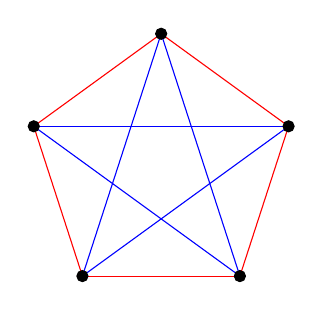
\begin{tikzpicture}
                \draw [red] (0,0) -- (2,0);
                \draw [red] (2,0) -- (2.618,1.9022);
                \draw [red] (2.618,1.9022) -- (1,3.0776);
                \draw [red] (1,3.0776) -- (-0.618,1.9022);
                \draw [red] (-0.618,1.9022) -- (0,0);

                \draw [blue] (0,0) -- (2.618,1.9022);
                \draw [blue] (0,0) -- (1,3.0776);
                \draw [blue] (2,0) -- (1,3.0776);
                \draw [blue] (2,0) -- (-0.618,1.9022);
                \draw [blue] (2.618,1.9022) -- (-0.618,1.9022);
        
                \filldraw (0,0) circle (2pt);
                \filldraw (2,0) circle (2pt);
                \filldraw (2.618,1.9022) circle (2pt);
                \filldraw (1,3.0776) circle (2pt);
                \filldraw (-0.618,1.9022) circle (2pt);
            \end{tikzpicture}
        
        \end{center}
        
        \caption{Graph of 5 vertices}
    \end{figure}
    Hence we see that there are no red triangles nor blue triangles, so no 
    monochromatic $K_3$. Hence $R(3,3)=6$.\cite{Greenwood1955}
\end{proof}

\textbf{Remark}: In the same paper \cite{Greenwood1955}, Greenwood and Gleason also proved the 
values of the following Ramsey numbers: $R(3,4)=9$, $R(3,5)=14$ and $R(4,4)=18$. 
As of the date of writing, only small Ramsey numbers are actually known exactly. 
$R(5,5)$ is unknown, although in 1995 McKay and Radziszowski proved that its 
value must lie between 43 and 49 inclusive \cite{McKay1995}. Its actual value is unknown,  
and the exact values of Ramsey numbers are often computed using algorithms, and very 
powerful computers. Using their bounds, even for a simple $2$-colouring, a 
computer would have to check at least $2^{43}\approx 8.8$ trillion different colour 
configurations of $K_5$.\\

Greenwood and Gleason also showed that $R_3(3,3,3)=17$, i.e. every complete graph 
of order at least 17 has a monochromatic $K_3$, when coloured with 
three colours. In fact, \autoref{prop:ram} holds for any finite $r$-colouring:

\begin{theorem}[Ramsey's Theorem for $r$-colours] \label{thr:ram2}

    Given $r$ positive integers, $s_1, s_2,\ldots, s_r$, there exist a least
    positive integer, $R_r(s_1,\ldots,s_r)$, such that any r-colouring of $K_n$ with 
    $n\geq R_r(s_1,\ldots,s_r)$ contains, as a clique, a monochromatic $K_{s_i}$
    for some $i\in\{1,\ldots r\}$, coloured by the $i^{\text{th}}$ colour.\label{thr:genRamsey}

\end{theorem}

\begin{proof}

    We again proceed by induction on $r$. The base case for $R_2(s_1,s_2)$ is
    true by the previous theorem. So we assume by induction that
    $R_{r-1}(s_1,\ldots ,s_{r-1})$ exists. Then in any $r$-colouring of $K_n$ we 
    replace the first two colours by a new colour. If $n$ is sufficiently large,
    then either there is a $K_{s_1}$ coloured with the $i^{\text{th}}$ colour for
    some $i \in \{3,\ldots,r\}$, or else for $m=R(s_1,s_2)$ there is a $K_m$
    coloured with the new colour. I.e. in the original colouring this $K_m$ is 
    coloured with the first two original colours. In the first case we are done,
    and in the second, for $i=1$ or 2, we can find a monochromatic $K_{s_i}$ in
    $K_m$ coloured in $K_m$ coloured with the $i^{\text{th}}$ colour. Hence,
    $$R_r(s_1,\ldots,s_r)\leq R_{r-1}(R(s_1,s_2),s_3,\ldots,s_r)$$

\end{proof}

Whilst we have been discussing Ramsey's theorem in a strictly graph-theoretical sense,
the theory extends beyond that. If we are given a set $V$ (which we 
have been referring to as the set of vertices of a given graph), so far we have been 
looking at partitioning (colouring) the set $V^{(2)}$ (the edges) into $r$ classes. 
However, \autoref{thr:ram2} still holds when we partition $V^{(k)}$ into $r$ classes, 
for any $k,r\in\Z^+$.

\begin{theorem}[Ramsey's Theorem] \label{thr:hyper}

    Given $r$ positive integers, $s_1, s_2,\ldots, s_r$, such that $1<k<\text\{min\}{s_1\ldots s_r}$, there exist a least
    positive integer, $R_r^{(k)}(s_1,\ldots,s_r)$, such that any $r$-colouring of $[n]^{(k)}$ 
    with $n\geq R_r^{(k)}(s_1,\ldots,s_r)$ contains, as a clique, a monochromatic 
    $[s_i]^{(k)}$ for some $i\in\{1,\ldots ,r\}$, coloured by the $i^{\text{th}}$ colour.  \cite{Ramsey1930}

\end{theorem}

\begin{proof}
    For simplicity will consider the case $r=2$. The proof is very similar to the 
    one for \autoref{prop:ram}, in that we use double induction on $s$ and $t$. 
    We will assume that both $R^{(k)}(s-1,t)$ and $R^{(k)}(s,t-1)$ exist, and 
    also $R^{(k-1)}(u,v)$ exists for all $u,v\in\Z^+$.\\

    Let $X$ be a set with $R^{(k-1)}(R^{(k)}(s-1,t),R^{(k)}(s,t-1))+1$ elements.
    Given any 2-colouring $\chi:X^{(k)}\to [2]$, choose any $x\in X$ and define 
    another 2-colouring $\chi':Y^{(k-1)}\to [2]$, where $Y=X\setminus\{x\}$, 
    given by $\chi'(\sigma) = \chi(\sigma\cup\{x\})$ for all $\sigma\in Y^{(k-1)}$. 
    By the definition of $R^{(k-1)}(u,v)$, we assume that $Y$ has a red (for $\chi'$) 
    subset $Z$ with $R^{(k)}(s-1,t)$\\

    Now we look at the restriction $\chi|_{Z^{(k)}}$. If it has a blue $t$-set, 
    then we are done, since $Z^{(k)}\subset X^{(k)}$, so a blue $t$-set of $Z$ 
    certainly also has a blue $t$-set of $X$. On the other hand, if there is no 
    blue $t$-set of $Z$ then there is a red $(s-1)$-set. The union of this red 
    $(s-1)$-set with $\{x\}$ is then a red $s$-set of $X$, since $\{x\}\cup\sigma$ 
    is red $\sigma\in Z^{(k-1)}$.\cite{Bollobas1998}
\end{proof}

\textbf{Remark}: We use the colour-grouping argument described in the proof of 
\autoref{thr:ram2} to prove that \autoref{thr:hyper} is in fact true for 
$r$-colourings. That is, $R_r^{(k)}(s_1,\ldots,s_r)$ exists.

\subsection{Infinite Graphs}
\label{sec:1.2}

The statement of Ramsey's theorem in the introduction, \cite{thr:Ramsey}
concerns partitioning a countably infinite set $\Gamma$ into $r$ disjoint 
subsets, where $r\in\Z^+$.

\begin{definition}[Infinite graph]

    We define the infinite complete graph, $K_\infty$, as the ordered pair
    $K_\infty:=(\Gamma,\Gamma^{(2)})$.

\end{definition}

\begin{theorem}[Ramsey's theorem for Infinite Graphs]\label{thm:ram}

    For any r-colouring of the edges of $K_\infty$, say
    $\chi :\Gamma^{(2)}\to\{c_1,\ldots, c_r\}$, there exists 
    within it a countably infinite monochromatic clique. In other words, there 
    exists $X \subset K_\infty$ such that $X$ is countably infinite, and $\chi|_{X^{(2)}}$ is the
    constant function.

\end{theorem}

\textbf{Remark}: It should be noted that whilst \autoref{thm:ram} is referring to 
the edges of the infinite graph, $\Gamma^{(2)}$, Ramsey's original theorem states 
that the same result holds for any $r$-colouring of $\Gamma^{(k)}$, for 
any $k,r \in \Z^+$. That is, we can always find a countably infinite monochromatic 
subset $\Delta \subset \Gamma$.

\begin{proof}

    Fix an arbitrary $a_1 \in \Z^+$. Then by the pigeonhole principal, 
    there must exist a countably infinite set $\mathcal{B}_1\subseteq\Z_+\setminus
    \{a_1\}$ such that all of the $a_1-\mathcal{B}_1$ edges (i.e. edges of the
    form $(a_1,b_1)$ with $b_1\in\mathcal{B}_1$ are of the same colour, say $c_1$.\\

    Now again fix an arbitrary $a_2\in\mathcal{B}_1$. Again, we find some countable
    $\mathcal{B}_2\subseteq\mathcal{B}_1$ such that all of the $a_2-\mathcal{B}_2$
    are of the same colour, say $c_2$.\\

    If we repeat this inductively, we obtain a sequence $a_1,a_2,\ldots$ 
    and a sequence of colours $c_1,c_2,\ldots$ such that $\chi(\{a_i,a_j\})=
    c_i$, for $i<j$.\\

    Now again by the pigeonhole principal, since there are finitely many colours,
    there exists an countable subsequence $c_{i_1}, c_{i_2}, \ldots$ that is 
    constant, i.e. each term is equal to $c_i$. Then $\{a_{i_1},a_{i_2}, \ldots\}$ is a
    monochromatic set, coloured by $c_i$.\cite{Narayana2017}

\end{proof}

An interesting corollary of this result is the following fundamental theorem from 
analysis:

\textbf{Corollary}: [Bolzano-Weierstrass Theorem]

Let $(x_i)_{i\in \Z_+}$ be a bounded sequence of real numbers. Then it has
a convergent subsequence.

\begin{proof}

    We define a 2-colouring of ${\Z^+}^{(2)}$ by calling $\{i,j\}$ \textit{red} 
    if $x_i <x_j$, and \textit{blue} if $x_i\geq x_j$.

    Then Ramsey's theorem for infinite graphs gives us a countably infinite monochromatic 
    set, which in this case is a monotone subsequence of $(x_i)$. And since it 
    is bounded, by the monotone convergence theorem it must converge.\cite{Narayana2017}

\end{proof}

%\newdimen\R
%\R=0.8cm
%
%\begin{tikzpicture}
%    % Indicate the boundary of the regular polygons
%    \draw [thin,black!20] circle (\R) ;
%    \fill[black!20] circle (2pt);
%    \draw (0:\R) \foreach \x in {120,240} {
%            -- (\x:\R)
%        } -- cycle (90:\R) node[above] {$n=3$} ;
%    \draw[xshift=2.5\R] (0:\R) \foreach \x in {90,180,...,359} {
%            -- (\x:\R)
%        } -- cycle (90:\R) node[above] {$n=4$} ;
%    \draw[xshift=5.0\R] (0:\R) \foreach \x in {72,144,...,359} {
%            -- (\x:\R)
%        } -- cycle (90:\R) node[above] {$n=5$} ;
%    \begin{scope}[yshift=-3\R]
%        \draw (0:\R) \foreach \x in {60,120,...,359} {
%                -- (\x:\R)
%            }-- cycle (90:\R) node[above] {$n=6$} ;
%            
%        % 360/7 = 51.4286 For PGF v < 1.18 we have to round to the nearest
%        % integer. Newer version support fractional angle values.
%        % For a more accurate result use the sequence
%        % {51, 103, 154, 206, 257, 309}
%        %
%        \draw[xshift=2.5\R] (0:\R) \foreach \x in {51.4286,102.8571,...,359} {
%                -- (\x:\R)
%            }-- cycle (90:\R) node[above] {$n=7$} ;
%        \draw[xshift=5.0\R] (0:\R) \foreach \x in {45,90,...,359} {
%                -- (\x:\R)
%            } -- cycle (90:\R) node[above] {$n=8$} ;
%    \end{scope}
%    \draw[yshift=-6.0\R] (0:\R) \foreach \x in {10,20,...,359} {
%            -- (\x:\R)
%        } -- cycle (90:\R) node[above] {$n=36$} ;
%\end{tikzpicture}
%
%
%
%%\subsection{Graph Ramsey Theory \cite{Bollobas1998}}
%%\label{sec:1.3}
%%
%%\begin{definition}[Isomorphism of Graphs]
%%
%%\end{definition}
%%
%\begin{definition}[Generalised Ramsey Number]
%
%\end{definition}
    